Główne założenia dotyczące tej pracy zostały przedstawione w drugim rozdziale tego raportu. W tym rozdziale przedstawiono konstrukcję obiektu regulacji temperatury oraz połączenie komponentów elektrycznych w funkcjonalną całość.

Celem tej pracy było stworzenie układu pomiarowo-regulacyjnego. Główną jednostką operacyjną jest płytka Arduino, pełniąca rolę sterownika kontrolującego wszystkie podzespoły oraz odpowiedzialnego za udostępnianie danych urządzeniom mobilnym.


\section{Wykorzystane podzespoły} 
W tym rozdziale przedstawiono podstawowe informację na temat najważniejszych wykorzystanych peryferiów.
\subsection{LCD}%%jest OK
\begin{figure}[H]
	\centering
	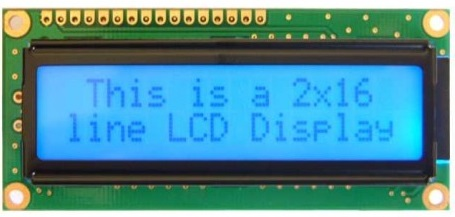
\includegraphics[scale=0.8]{lcd2x16.jpg}
	\caption{Ekran LCD 2x16 znaków}
\end{figure}
Do wyświetlania danych wybrano popularny wyświetlacz LCD 2x16 znaków, ze sterownikiem HD44780, odpowiedzialnym za wyświetlanie odebranych danych. Moduł zasilany jest napięciem 5V i może być sterowany w 4 trybach:
\begin{itemize}
\item 8-bitowym bez odczytu flagi zajętości,
\item 8-bitowym z odczytem flagi zajętości,
\item 4-bitowym z odczytem flagi zajętości,
\item 4-bitowym bez odczytu flagi zajętości.
\end{itemize}
Ze względu na ograniczoną ilość pinów Arduino zdecydowano się na wykorzystanie ostatniego z wymienionych trybów.

 \begin{table}[H]
	\centering
	\caption{Opis pinów ekranu LCD}
	\begin{tabular}{|c|c|c|}
		
  \hline 
  \bfseries Nr & \bfseries Nazwa & \bfseries Opis \\
  \hline
  1&VSS&Masa  \\
  \hline
  3&V0&Kontrast  \\
  \hline
  4&RS&Wybór rejestru instrukcji wyświetlacza (stan niski)\\
   &&albo rejestru danych (wysoki) \\
  \hline
  5&R/W& Odczyt (stan niski)/ Zapis (stan wysoki)  \\
  \hline
    6&E& Odblokowanie wyświetlacza  \\
  \hline
      7-14&DB0-7& Magistrala danych  \\
  \hline
        15&LEDA& Zasilanie podświetlania +5V  \\
  \hline
        16&LEDK& Masa podświetlenia  \\
  \hline
\end{tabular}
\end{table}

\subsection{DS18B20}
DS18B20 to popularny termometr cyfrowy wyposażony w interfejs komunikacyjny 1-wire. Podjęto decyzję o wykorzystaniu tego komponentu, dlatego że oferował on wystarczająco dużą dokładność pomiarową i możliwość poznania wcześniej nieznanego autorowi protokołu komunikacyjnym.
\begin{figure}[H]
	\centering
	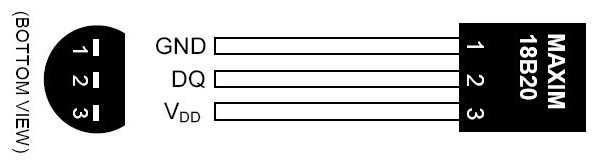
\includegraphics[scale=0.65]{ds18b20.jpg}
	\caption{Opis wyprowadzeń czujnika temperatury DS18B20}
\end{figure}
Termometr cyfrowy DS18B20 posiada jedynie trzy wyprowadzenia:
\begin{itemize}
\item VDD- napięcie zasilania mogące wynosić od 3V do 5,5V,
\item DQ- sygnał cyfrowy,
\item GND- masa układu.
\end{itemize}
Przedstawiony termometr pozwala na mierzenie temperatury w zakresie $-55^{\circ} C$ do $125^{\circ} C$. Rozdzielczość termometru może zostać dostosowana przez użytkownika, poprzez wybranie ilości otrzymywanych bitów danych. Istnieje możliwość wyboru trybu 9, 10, 11, 12 bitowego, odpowiadającego wartościom 0.5, 0.25, 0.125 i 0.625 stopnia Celsjusza. Zdecydowano się na wybór trybu 12 bitowego, w celu poprawy działania regulatora. Na wyświetlaczu oraz urządzeniu mobilnym wartość została zaokrąglona do jednego miejsca po przecinku.
%\subsection{Termometr LM35}%%jest OK
%\begin{figure}[H]
%	\centering
%	\includegraphics[scale=0.5]{lm35.jpg}
%	\caption{Termometr LM35}
%\end{figure}
%LM35DZ to analogowy czujnik temperatury, którego wyjście przyjmuje wartość napięcia proporcjonalną do zmierzonej temperatury. Termometr działa w zakresie temperatur od 90 do 100 stopni Celsjusza. Czujnik został fabrycznie skalibrowany do mierzenia temperatury w stopniach Celsjusza. Dokładność pomiaru wynosi około 0,5 C.
%
%Termometr cyfrowy LM35 posiada jedynie trzy wyprowadzenia:
%\begin{itemize}
%\item VDD- napięcie zasilania mogące wynosić od 4V do 30V
%\item OUT- sygnał analogowy,
%\item GND- masa układu.
%\end{itemize}
\subsection{Moduł Bluetooth HC-06}%%jest OK

W fazie powstawania pierwotnej koncepcji projektu zastanawiano się nad wyborem sposobu komunikacji bezprzewodowej między mikrokontrolorem, a urządzeniem mobilnym z oprogramowaniem Android. Rozważanymi technologiami był moduł XBee oraz moduł Bluetooth. Ze względu na cenę modułów oraz wymaganą ilość wejść/wyjść mikrokontrolera zdecydowano się na zakup modułu Bluetooth HC-06, pozwalającego na pracę pinów danych w logice 5V..
\begin{figure}[H]
	\centering
	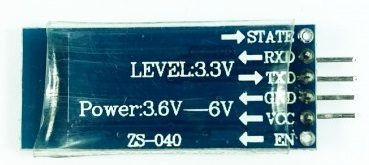
\includegraphics[scale=0.5]{hc06.jpg}
	\caption{Moduł Bluetooth HC-06}
\end{figure}
Charakterystycznymi cechami wybranego modułu jest zasięg do około 10m i fabrycznie ustawiony tryb slave, bez możliwości przejścia w tryb master (inicjacja połączenia między modułami), którym w tym przypadku jest telefon komórkowy lub tablet. Moduł przekazuje dane z prędkością 9600 bitów na sekundę.

\begin{table}[H]
	\centering
	\caption{Opis wejść/wyjść modułu Bluetooth HC-06}
	\begin{tabular}{|c|c|c|}
		
  \hline 
 \bfseries Nr & \bfseries Nazwa & \bfseries Opis \\
  \hline
  1&STATE& Informacja o połączeniu z innym urządzeniem  \\
  \hline
  2&RXD& Komunikacja szeregowa  \\
  \hline
  3&TXD& Komunikacja szeregowa \\
  \hline
  4&GND& Masa układu \\
  \hline
    5&VCC& Zasilanie  \\
  \hline
      6&EN&Pin pozwalający na włączenie trybu konfiguracji modułu \\
  \hline
\end{tabular}
\end{table}
\subsection{L293D}%%jest OK
\begin{figure}[H]
	\centering
	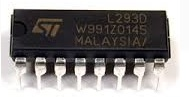
\includegraphics[scale=0.65]{l293d.jpg}
	\caption{Sterownik silników L293D}
\end{figure}
L293D to dwukanałowy sterownik silników o napięciu zasilania do 36V. Moduł zazwyczaj określany jest jako mostek H, ale w rzeczywistości składa się z czterech połowicznych mostków H. Charakteryzują się one tym, że posiadają tylko dwa tranzystory po jednej stronie obciążenia. Sterownik pozwala na zasilenie urządzenia o średnim poborze prądu o wartości 0,6A, a nawet do 1,2A w przypadku pracy krótkotrwałej. Moduł chroniony jest przez obudowę DIP z wyprowadzonymi 16 nóżkami. Moduł został wykorzystany do sterowania dwoma silnikami DC o napięciu znamionowym 12V.
\begin{table}[H]
	\centering
	\caption{Opis wejść/wyjść L293D}
	\begin{tabular}{|c|c|c|}
		
  \hline 
 \bfseries Nr & \bfseries Nazwa & \bfseries Opis \\
  \hline
    1&ENABLE1&Sygnał sterujący(PWM) kanału pierwszego \\
  \hline
      2,7&INPUT1-2&Kierunek kanału pierwszego  \\
  \hline
  3,6&OUTPUT1-2&Wyjście kanału pierwszego  \\
  \hline
           8&VS&Zasilanie silników  \\
  \hline
    9&ENABLE2&Sygnał sterujący(PWM) kanału drugiego \\
  \hline
       10,15&INPUT3-4&Kierunek kanału drugiego  \\
  \hline
  11,14&OUTPUT3-4&Wyjście kanału drugiego  \\
  \hline
       16&VSS&Zasilanie części logicznej  \\
  \hline
           4,5,12,13&GND&Masa układu  \\
  \hline
\end{tabular}
\end{table}
\newpage
\subsection{DFRobot - dwukanałowy sterownik silników }%%jest OK

\begin{figure}[H]
	\centering
	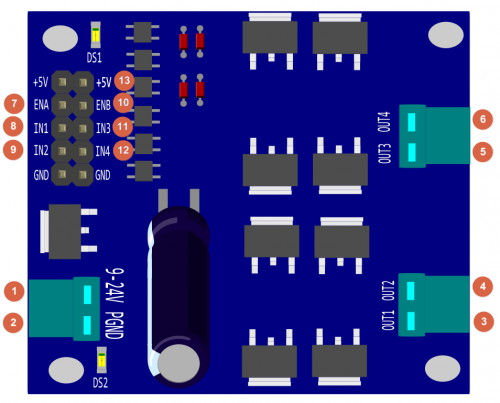
\includegraphics[scale=0.5]{dfrobot.jpg}
	\caption{Sterownik silników DFRobot}
\end{figure}
Moduł DFRobot to dwukanałowy sterownik silników prądu stałego. Urządzenie powinno zostać zasilone napięciem od 6,5 do 27V. Pozwala na zasilenie silnika o średnim poborze prądu do 7 A, a w przypadku wartości chwilowych aż do 50 A. Sterownik ten został wybrany ze względu na dużą moc i dwukanałowość, która mogłaby okazać się potrzebna w sytuacji gdy jedno ogniwo byłby za słabe by znacznie wpływać na temperaturę w obiekcie. Układ pracuje w logice 3,3 V oraz 5V. Sterowanie modułem przebiega w ten sam sposób jak w przypadku sterownika L293D, na dwa piny sterujące podajemy odpowiednią kombinację 0 i 1 logicznej, tym samym wyznaczając kierunek obrotów, a następnie na kolejnym pinie zadajemy prędkość wykorzystując sygnał PWM.
\begin{table}[H]
	\centering
	\caption{Opis wejść/wyjść sterownika DFRobot}
	\begin{tabular}{|c|c|c|}
		
  \hline 
  \bfseries Nr & \bfseries Nazwa & \bfseries Opis \\
  \hline
    1&9-24V&Napięcie zasilania \\
  \hline
     2&IPGND&Masa układu  \\
  \hline
  3,4&OUT1/2&Wyjście 1/2 kanału A  \\
  \hline
           5,6&OUT3/4&Wyjście 1/2 kanału B  \\
  \hline
    7&ENA&PWM dla kanału A \\
  \hline
       8,9&IN1/2&Wejście sterujące 1/2 kanału A  \\
  \hline
  10&ENB&PWM dla kanału B  \\
  \hline
       11,12&IN3/4&Wejście sterujące 1/2 kanału B  \\
  \hline
           13&+5V&Napięcie referencyjne: 3,3V lub 5V  \\
  \hline
\end{tabular}
\end{table}
\subsection{Ogniwo Peltiera TEC-12706}%%jest OK
Ogniwo Peltiera zostało szerzej opisane na we wstępie teoretycznym do pracy. W opisanym projekcie użyto ogniwa Peltiera zasilanego napięciem 12V (do 15V) oraz o średnim poborze prądu wynoszącym 4,5A (maksymalnym 6A).
\begin{figure}[H]
	\centering
	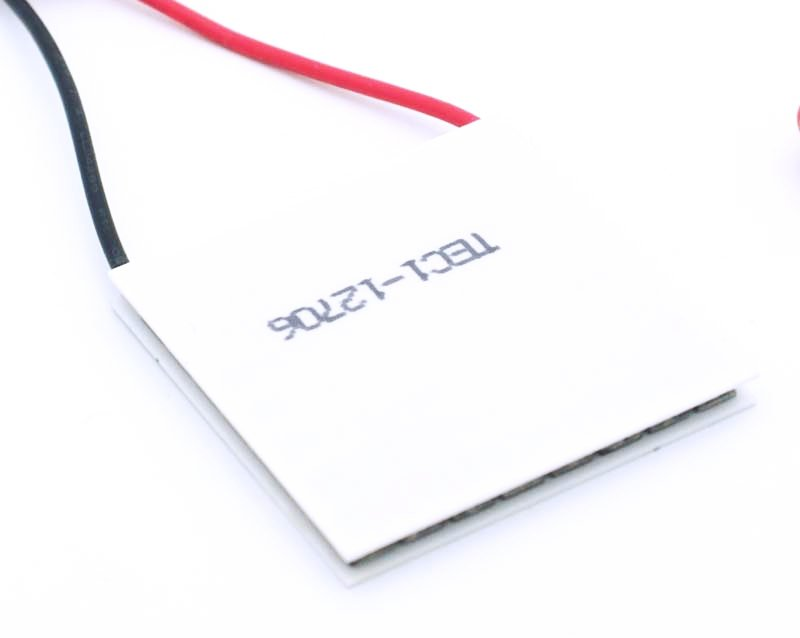
\includegraphics[scale=0.15]{tec12706.jpg}
	\caption{Moduł ogniwa Peltiera (wym. 40x40x3,8 mm)}
\end{figure}
Ogniwo to charakteryzuje się maksymalną mocą wejściową około 90W i mocą odprowadzania ciepła do 53,3W. Sprawność ogniwa zależy od szczelności termicznej chłodzonego/ogrzewanego obiektu. Zdecydowano się na wybór takiego ogniwa ze względu na łatwo dostępne źródło zasilania, pozwalające na osiągnięcie maksymalnej mocy ogniwa. Jest to wersja ogniwa najczęściej wykorzystywana w lodówkach turystycznych, popularna ze względu na możliwość zasilenia przez gniazdko zapalniczki samochodowej.

\subsection{Wiatrak komputerowy- silnik DC}%%jest OK
Ze względu na szeroki zakres dostępu do starych komponentów komputerowych wybrano wiatraki wykorzystywane do chłodzenia procesorów. Silnik charakteryzuje się napięciem znamionowym 12V i poborem prądu o wartości 0,6A. W początkowej fazie projektu używano wiatraka promieniowego, ale ze względu na duży hałas podczas pracy podjęto decyzje o wymianie na wiatrak komputerowy. Silnik może obracać się z prędkością od 2500 do 3400 obrotów na minutę.
\begin{figure}[H]
	\centering
	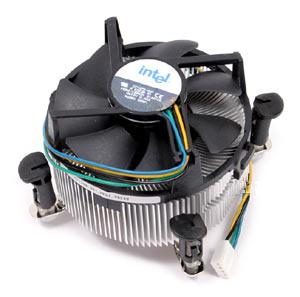
\includegraphics[scale=0.6]{wiatrakDC.jpg}
	\caption{Wykorzystany wiatrak (bez radiatora)}
\end{figure}
Każdy z wiatraków posiada 3 piny:
\begin{itemize}
\item 1- napięcie zasilania silnika,
\item 2- uziemienie układu,
\item 3- sygnał z halotronu.
\end{itemize}

\subsection{Zasilacz ATX}
Do zasilenia układu wykorzystano zasilacz ATX firmy MODECOM o mocy 350W. Układ został wykorzystany ze względu na fakt, że był dostępny po rozebraniu na części starego komputera stacjonarnego autora. Dodatkową zaletą okazały się wyprowadzenia zasilania na 5 V, użyte do uruchomienia Arduino oraz wyjścia 12 V, wykorzystane do zasilenia wiatraków i ogniwa Peltiera.
\begin{figure}[H]
	\centering
	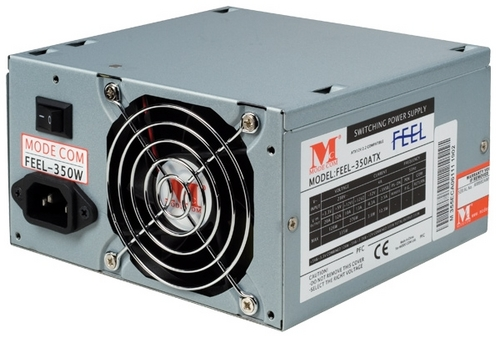
\includegraphics[scale=0.4]{modecom.jpg}
	\caption{Zasilacz ATX}
\end{figure}
\section{Obiekt pomiarowy}%%jest OK
\begin{figure}[H]
	\centering
	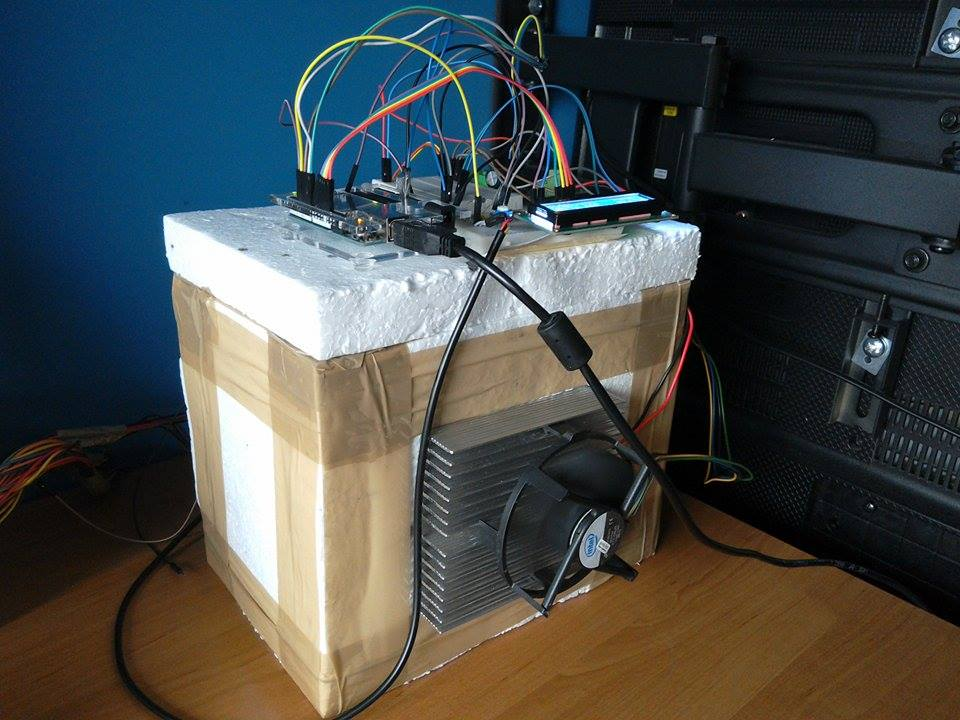
\includegraphics[scale=0.25]{stanowisko.jpg}
	\caption{Obiekt regulacji temperatury}
\end{figure}
Podczas konstruowania obiektu pomiarowego za najważniejsze czynniki konstrukcyjne przyjęto: izolację termiczną materiału z którego zostanie wykonany, łatwość modelowania go oraz koszty wykorzystania. Dlatego zdecydowano się na styropian do ocieplania fasad. Cechy te okazały się bardzo korzystne ze względu na fakt, że rozmiar i wygląd "pomieszczenia" był kilkukrotnie modyfikowany z powodów takich jak zbyt słabe uszczelnienie czy też zbyt duży rozmiar obiektu niepozwalający na znaczny wpływ ogniwa Peltiera na temperaturę w obiekcie w rozsądnym przedziale czasowym. Ostateczna konstrukcja przyjęła postać styropianowego prostopadłościanu.

Kolejną częścią, która wymagała przemyślenia było miejsce i sposób zamontowania ogniwa Peltiera, tak by mogło ono optymalnie chłodzić i ogrzewać pomieszczenie. Ogniwo zostało zamontowane na bocznej ścianie. Dodatkowym powodem przemawiającym za takim rozwiązaniem było wolne miejsce na dachu, w którym zamontowano Arduino i pozostałe podzespoły.

Ze względu na dużą ilość wydzielanego ciepła ze strony ciepłej podczas chłodzenia obiektu, ogniwo musiało zostać przymocowane do dużych radiatorów z obu stron. Do części ogniwa bezpośrednio wpływającej na wnętrze obiektu przymocowano najpierw aluminiowy blok, a następnie radiator. Takie rozwiązanie zastosowano w celu ograniczenia wpływu temperatury radiatora znajdującego się na zewnątrz na część wewnętrzną. 

Jednak nawet takie rozwiązanie okazało się nie być pozbawione wad. Przy długotrwałym chłodzeniu obiektu, strona gorąca nagrzewała się tak bardzo, że różnica temperatury pomiędzy dwoma stronami ogniwa była zbyt duża, co powodowało stopniowe nagrzewanie się strony chłodzącej. Sytuacja taka wynika z tego, że różnica temperatur między stroną ciepłą a zimną ma swoją wartość maksymalną, po przekroczeniu której dochodzi do ogrzania części chłodnej, w celu zmniejszenia różnicy temperatur. 
Skutecznym rozwiązaniem tego problemu okazało się dołączenie wiatraczka komputerowego do każdego z radiatorów. Zabieg ten poprawił prędkość oddawania temperatury do powietrza oraz jego cyrkulację w obiekcie, w wyniku czego procesy regulacji temperatury stały się dynamiczniejsze. Ostatnim elementem konstrukcji jest termometr, który został wprowadzony do środka obiektu poprzez jedną z bocznych ścian.

\section{Układ wykonawczy}
Główną jednostką obliczeniową układu jest Arduino, do którego zostały podłączone podzespoły składające się na:
\begin{itemize}
\item sterownik silników DFRobot,
\item ogniwo Peltiera,
\item dwukanałowy sterownik silników L293D,
\item 2 silniki DC,
\item ekran LCD 2x16,
\item termometr analogiczny LM35,
\item moduł Bluetooth HC-06,
\end{itemize}
których obsługa została szerzej opisana w kolejnym rozdziale.
Do podłączenia układu wykorzystano 800 stykową płytkę prototypową, na której umieszczono ekran LCD i pozostałe mieszczące się moduły. Komponenty zostały połączone zgodnie z opisami pinów i zaleceniami zawartymi w dokumentacji producentów. Na poniższym rysunku można zobaczyć schemat połączeń urządzeń.

\begin{figure}[H]
	\centering
	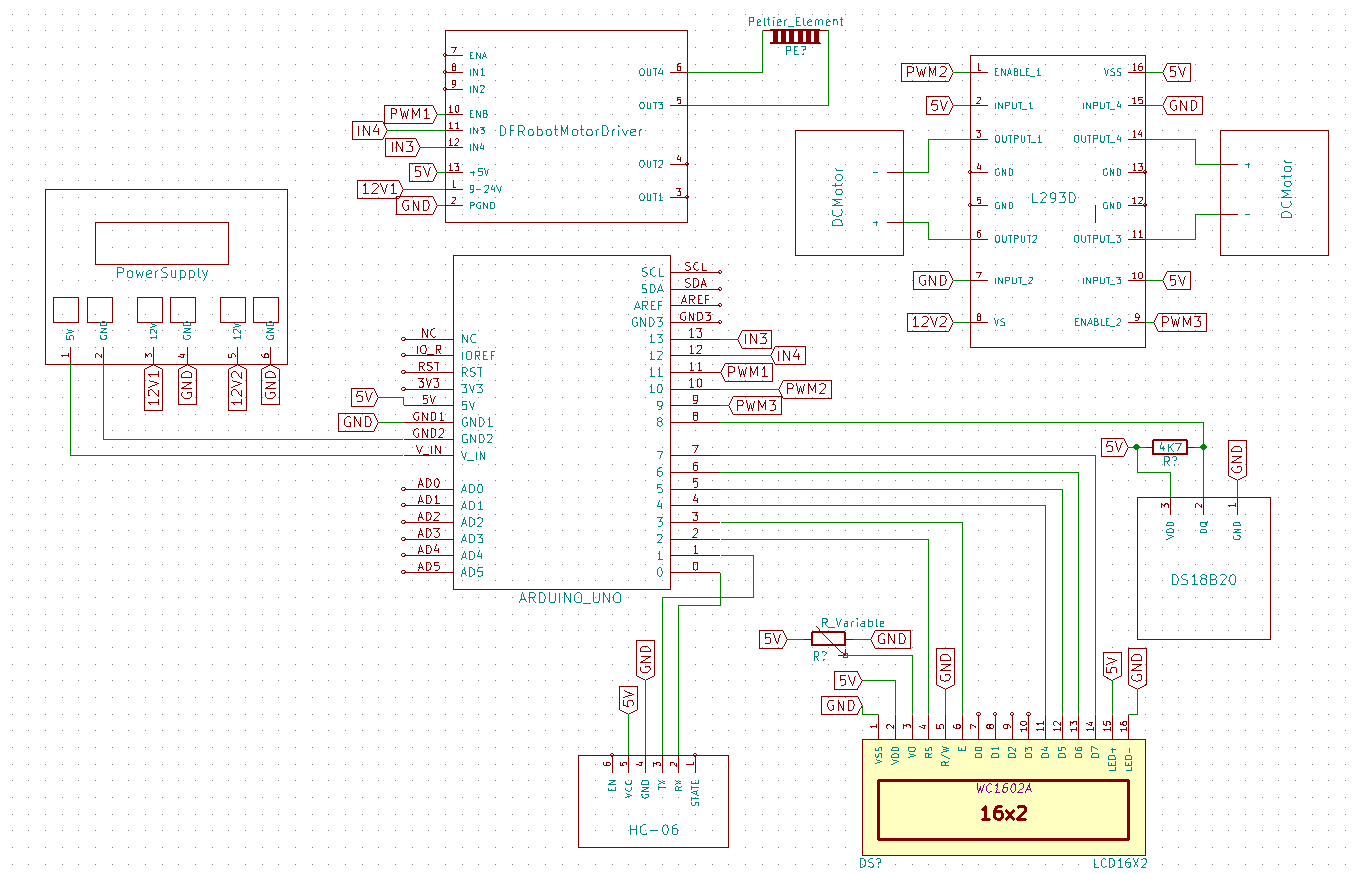
\includegraphics[scale=0.4]{schemat.png}
	\caption{Schemat połączeń elektrycznych}
\end{figure}

